\expandafter\def\csname ver@breakurl.sty\endcsname{2013/04/10}\expandafter\def\csname opt@breakurl.sty\endcsname{hyphenbreaks}% skip breakurl (dvips only); Tectonic runs XeTeX
\documentclass[sn-mathphys-num]{sn-jnl}
% Shared preamble for the Springer Nature (sn-jnl) versions: papers A and B. Load right after \documentclass{sn-jnl}.
\usepackage{amsmath,amssymb}
\usepackage{graphicx}
\usepackage{booktabs}
\usepackage{tabularx}
\usepackage{array}
\usepackage{xcolor}
\usepackage{tikz}
\usetikzlibrary{arrows.meta,positioning,fit,backgrounds,calc,shapes.geometric,shapes.misc}
\graphicspath{{../figures/}}
% sn-jnl loads breakurl, which expects pdfTeX/dvips; Tectonic runs XeTeX
\makeatletter\def\headerps@out#1{}\makeatother
\AtBeginDocument{\def\doi#1{\url{https://doi.org/#1}}}\providecommand\burl{\url}
% a result the overnight runs have not produced yet (papers/analysis/new_results.py fills it in)
\newcommand{\pending}{\textcolor{red}{[pending]}}
% a step that needs people (raters, reviewers, ethics); see papers/HUMAN_STUDIES.md
\newcommand{\humanpending}[1]{\textcolor{red}{[#1]}}
\tikzset{
  >={Stealth[length=1.8mm]},
  box/.style={draw, rounded corners=2pt, align=center, font=\scriptsize, minimum height=7mm, inner sep=2pt, fill=#1},
  box/.default=cyan!8,
  decision/.style={draw, diamond, aspect=2.2, align=center, font=\scriptsize, inner sep=1pt, fill=yellow!12},
  state/.style={draw, circle, align=center, font=\scriptsize, minimum size=12mm, fill=#1},
  state/.default=cyan!8,
  lab/.style={font=\tiny, align=center},
}
\newcolumntype{Y}{>{\raggedright\arraybackslash}X}

\newcommand{\numCasFalse}{3.7\%}
\newcommand{\numCasRisk}{93.5\%}
\newcommand{\numCasShare}{63\%}
\newcommand{\numCompCIPzero}{[0.969, 0.987]}
\newcommand{\numCompCIVzero}{[0.954, 0.979]}
\newcommand{\numCompCIVtwo}{[0.956, 0.982]}
\newcommand{\numCompPzero}{0.978}
\newcommand{\numCompVzero}{0.967}
\newcommand{\numCompVtwo}{0.970}
\newcommand{\numDiffPzero}{$-0.008$ [$-0.022$, $+0.004$]}
\newcommand{\numFilterDropped}{240}
\newcommand{\numFilterTotal}{533}
\newcommand{\numJailPzero}{6}
\newcommand{\numJailVzero}{1}
\newcommand{\numJailVtwo}{0}
\newcommand{\numLLMfalse}{4.8\%}
\newcommand{\numLLMmsMed}{416}
\newcommand{\numLLMmsNinety}{736}
\newcommand{\numLLMrisk}{94.8\%}
\newcommand{\numLeaksPzero}{4}
\newcommand{\numLeaksVzero}{0}
\newcommand{\numLeaksVtwo}{1}
\newcommand{\numPortPzero}{0}
\newcommand{\numPortVzero}{0}
\newcommand{\numPortVtwo}{0}
\newcommand{\numRPmissNoRecPzero}{66.7\%}
\newcommand{\numRPmissNoRecVzero}{55.3\%}
\newcommand{\numRPmissNoRecVtwo}{69.8\%}
\newcommand{\numRPmissRecPzero}{51.8\%}
\newcommand{\numRPmissRecVzero}{21.0\%}
\newcommand{\numRPmissRecVtwo}{24.4\%}
\newcommand{\numRPmissPzero}{55.8\%}
\newcommand{\numRPmissVzero}{43.3\%}
\newcommand{\numRPmissVtwo}{36.8\%}
\newcommand{\numRPnPzero}{231}
\newcommand{\numRPnVzero}{231}
\newcommand{\numRPnVtwo}{231}
\newcommand{\numSIfailPzero}{1}
\newcommand{\numSIfailVzero}{0}
\newcommand{\numSIfailVtwo}{0}
\newcommand{\numTurnsPzero}{294}
\newcommand{\numTurnsVzero}{294}
\newcommand{\numTurnsVtwo}{294}
\newcommand{\numWGemmaDep}{47.5\%}
\newcommand{\numWGemmaLLM}{91.5\%}
\newcommand{\numWQwenDep}{58.9\%}
\newcommand{\numWQwenLLM}{87.7\%}


\begin{document}

\title[Recognising Reworded Risk Questions]{Recognising Reworded Risk Questions in a Simulated Psychiatric Patient: A Blind Benchmark,
Small Encoders, BM25 and a Zero-Shot Language Model}

% Author checks still to do: papers/HUMAN_STUDIES.md
\author*[1]{\fnm{Faaz Khan} \sur{Mohammad}}\email{faazkhn1000@gmail.com}
\author[1]{\fnm{Sanket} \sur{Salvi}}\email{sanket.salvi@mitwpu.edu.in}
\affil[1]{\orgdiv{Department of Computer Engineering and Technology}, \orgname{Dr.~Vishwanath~Karad MIT World Peace University}, \orgaddress{\city{Pune}, \state{Maharashtra}, \country{India}}}

\abstract{A simulated psychiatric patient must recognise when a student asks about suicidal thoughts, plans, means or other risk, however the
question is worded, because a missed question can make the patient deny something it should disclose. We built a blind benchmark of 512 doctor
questions over four cases, written from what each memory means by a writer that never saw the matching rules, and split by checksum into a
tuning half and a test half. On the test half, keyword tags found 35.1\% of risk questions; a hybrid of tags and a 33-million-parameter
sentence encoder, run on the processor in a few milliseconds, found 72.7\% while wrongly matching 15.2\% of non-risk questions. Five small
encoders and BM25 over the same example questions gave overlapping threshold-free results (area under the receiver operating characteristic curve 0.86--0.91 for risk), so the encoder choice was
not the bottleneck. The same 4-billion-parameter model that voices the patient, used as a zero-shot classifier, found \numLLMrisk{} of risk
questions with \numLLMfalse{} wrong matches, at a median of \numLLMmsMed\,ms per question; screening with the hybrid first kept \numCasRisk{}
recall while sending \numCasShare{} of questions to the model. Tuning cut-offs for recall alone was unsafe, and a classifier trained on
model-generated labels lost to simple rules. On two further test sets written by other local models, the deployed rules found \numWQwenDep{} and \numWGemmaDep{} of risk questions
and the zero-shot model \numWQwenLLM{} and \numWGemmaLLM. Inside conversations, missed matches became missed disclosures.}

\keywords{semantic matching, paraphrase, sentence embeddings, suicide risk assessment, simulated patients, benchmark}

\maketitle

\section{Introduction}\label{sec:intro}
In the Rapport simulator, a spoken standardised patient for psychiatry teaching described in a companion manuscript by the same authors, keyword matching caused every serious bug
found during evaluation. ``Thoughts that life \emph{isn't} worth living'', ``wishing you \emph{wouldn't} wake up'' and ``tablets or anything at
home'' each missed the memory they asked about, and one of these misses let the patient deny a passive death wish it should have disclosed.
Adding keywords fixed each case, but there is no end to the ways people phrase a question.

The patient's memories are trust-locked: an item may be shared only once the patient trusts the student enough. Matching a student's question
to these memories is unusual in three ways. It must be fast and local, because it runs on every spoken turn on the same laptop as a language
model and a voice. It must not leak: the text of a locked memory must never reach the language model or the user. And its two mistakes cost
different things. Missing a suicide question can suppress a required disclosure; wrongly matching an innocent question to a suicide memory makes
the patient evasive about something harmless, or invites it to talk about suicide when asked about sleep.

\textbf{Contributions.}
\begin{enumerate}
\item A blind benchmark of 512 doctor questions with a strict tuning/test split, labelled with the memories each asks about (Section~\ref{sec:bench}).
\item A hybrid matcher with trust locks applied after matching, a stricter ``clearly asked'' level for anything with consequences, and
training-free hand-set heads (Section~\ref{sec:method}).
\item A comparison with BM25, five small sentence encoders and the patient's own language model as a zero-shot classifier, with threshold-free
metrics and bootstrap intervals, and a cascade of the hybrid and the model (Section~\ref{sec:results}).
\item Two negative results: tuning for recall alone made the patient unsafe, and a classifier trained on noisy generated labels lost to simple
rules; and a measure of what missed matches cost inside conversations.
\end{enumerate}

\section{Related Work}\label{sec:related}
\textbf{Sentence embeddings and retrieval.} Sentence-BERT made it practical to compare sentences by meaning \cite{reimers2019sentencebert};
MiniLM showed that small distilled models keep most of the quality \cite{wang2020minilm}; contrastive training (SimCSE, E5, the BGE family) is the
standard recipe for small general-purpose encoders \cite{gao2021simcse,wang2022e5,xiao2023cpack}. Dense retrieval matches questions to
passages the same way \cite{karpukhin2020dpr}, and BEIR and MTEB showed that retrieval quality varies by domain and must be measured in the
target domain \cite{thakur2021beir,muennighoff2022mteb}; lexical BM25 \cite{robertson2009bm25} remains a strong baseline there. PAWS showed that
models trained on easy paraphrase pairs fail on pairs that share words but differ in meaning \cite{zhang2019paws}; our problem is the reverse,
questions that share no words but mean the same.

\textbf{Memory in simulated patients.} PatientAct gives each memory a trust level and activation cues \cite{sabour2026patientact}; AIPatient
retrieves from a knowledge graph built from health records, with several agents per turn \cite{yu2024simulated}; Patient-Zero checks replies against
single facts \cite{lai2025patientzero}; generative agents retrieve memories by recency, importance and relevance \cite{park2023generative}. These
systems report conversation quality, but none that we found reports how well the matching step survives rewording, or what it costs on a risk
topic.

\section{The Benchmark}\label{sec:bench}

\begin{figure}[t]
\centering
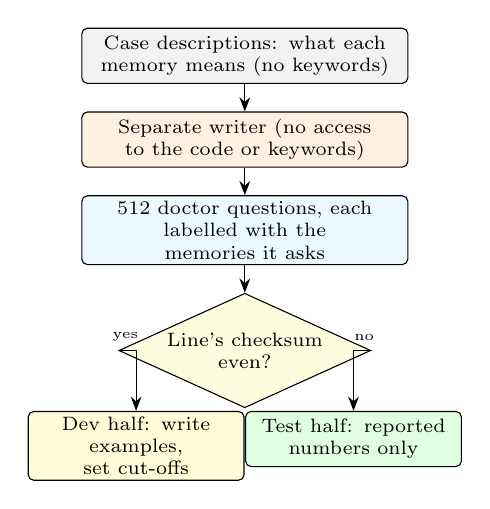
\begin{tikzpicture}[node distance=3.5mm]
\tikzset{b/.style={box=#1, text width=40mm}}
\node[b=gray!10] (a) {Case descriptions: what each\\memory means (no keywords)};
\node[b=orange!12, below=of a] (b) {Separate writer (no access\\to the code or keywords)};
\node[b=cyan!8, below=of b] (c) {512 doctor questions, each\\labelled with the memories it asks};
\node[decision, below=of c] (d) {Line's checksum\\even?};
\node[b=yellow!15, below left=4mm and -8mm of d, text width=26mm] (dev) {Dev half: write\\examples, set cut-offs};
\node[b=green!12, below right=4mm and -8mm of d, text width=26mm] (test) {Test half: reported\\numbers only};
\draw[->] (a) -- (b); \draw[->] (b) -- (c); \draw[->] (c) -- (d);
\draw[->] (d) -| node[lab, above, pos=0.2]{yes} (dev); \draw[->] (d) -| node[lab, above, pos=0.2]{no} (test);
\end{tikzpicture}
\caption{How the blind benchmark was built and split.}
\label{fig:bench}
\end{figure}

A writer (an AI agent with no access to the code) was given only a description of each case's memories: who the patient is, the kind of each
memory, and what the patient knows (Fig.~\ref{fig:bench}). It was asked to write questions a real doctor might ask about each memory: at least four
per memory and twelve per risk memory; a mix of textbook, gentle and indirect, clumsy, colloquial Indian English and euphemistic wording; most
lines free of the memory's own key words; every line understandable on its own; and some ``none'' lines (greetings, small talk, pure empathy)
that ask about nothing (Appendix~\ref{app:writer}). It confirmed it read nothing else.

The result has 512 lines over four cases, including 38 ``none'' lines; the writer marked 249 as hard (Table~\ref{tab:benchstats}). Labels are
narrow: a matcher that also returns a neighbouring memory is not penalised on recall, but the extras count as wrong matches. The split uses the
CRC-32 checksum of each line: even lines form the \emph{dev} half, which may be used for anything; odd lines form the \emph{test} half, used only
for reported numbers.

\begin{table}[t]
\caption{The benchmark by case}
\label{tab:benchstats}
\footnotesize
\begin{tabular*}{\linewidth}{@{\extracolsep{\fill}}lcccc@{}}
\toprule
Case & Lines & ``None'' & Marked hard & Risk pairs\\
\midrule
Depression & 176 & 10 & 89 & 41\\
Alcohol withdrawal & 154 & 10 & 77 & 55\\
Ward: wants to go home & 104 & 9 & 52 & 41\\
Ward: refuses tablets & 78 & 9 & 31 & 15\\
\midrule
Total & 512 & 38 & 249 & 152\\
\bottomrule
\end{tabular*}
\end{table}

\textbf{Measures.} \emph{Recall} is the share of (question, expected memory) pairs where the memory is found. \emph{Risk recall} counts only risk
memories (suicidal thoughts, plans, means, withdrawal fits, anger at home): 77 pairs in the test half. \emph{Risk false hits} is the share of
questions that ask about no risk memory but are matched to one. For threshold-free comparison every method scores every (question, memory)
pair of the question's case; we report the area under the ROC curve (AUROC) and the average precision (AUPRC) over the risk-memory pairs and over
all pairs, with 95\% intervals from 1,000 bootstrap resamples of test-half questions.

\textbf{Threats, and two more writers.} One AI writer produced both halves, and the dev half was used twice (to write example questions and to
set cut-offs). The test half therefore measures new wording, not a new writer. To test a new writer without human participants, two local models
from different families each wrote a further test set from the same memory descriptions and instructions (Appendix~\ref{app:writer}), with about
one line in four in code-mixed Hindi--English (Hinglish): Qwen3.5-4B and Gemma 4 E2B. Each shares something with a compared method (a Qwen model
wrote the generated probes; a larger Gemma is the zero-shot classifier), so a result counts only if it holds on both. These sets are used once,
with every cut-off still taken from the original dev half. Their labels come from the writer models and were not checked by a person.

\section{Methods}\label{sec:method}

\begin{figure}[t]
\centering
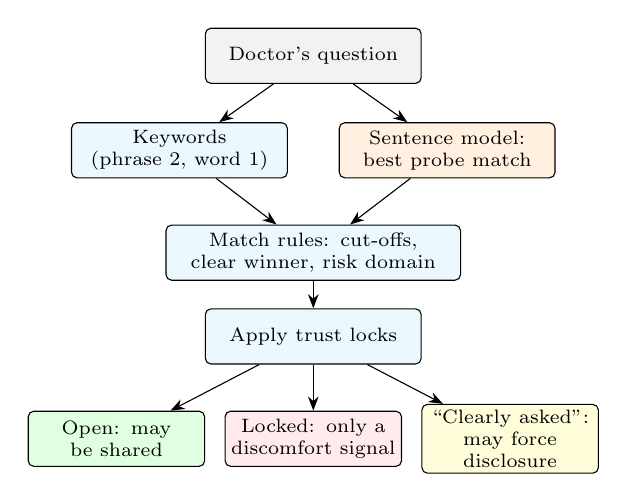
\begin{tikzpicture}[node distance=3.5mm and 4mm]
\tikzset{b/.style={box=#1, text width=26mm}}
\node[b=gray!10] (q) {Doctor's question};
\node[b=cyan!8] (lex) at ($(q)+(-17mm,-12mm)$) {Keywords\\(phrase 2, word 1)};
\node[b=orange!12] (emb) at ($(q)+(17mm,-12mm)$) {Sentence model:\\best probe match};
\node[b=cyan!8, text width=36mm] (rule) at ($(q)+(0,-25mm)$) {Match rules: cut-offs,\\clear winner, risk domain};
\node[b=cyan!8, below=of rule] (lock) {Apply trust locks};
\node[b=green!12, text width=21mm] (open) at ($(lock)+(-25mm,-13mm)$) {Open: may\\be shared};
\node[b=red!8, text width=21mm] (locked) at ($(lock)+(0,-13mm)$) {Locked: only a\\discomfort signal};
\node[b=yellow!15, text width=21mm] (strong) at ($(lock)+(25mm,-13mm)$) {``Clearly asked'':\\may force disclosure};
\draw[->] (q) -- (lex); \draw[->] (q) -- (emb); \draw[->] (lex) -- (rule); \draw[->] (emb) -- (rule); \draw[->] (rule) -- (lock);
\draw[->] (lock) -- (open); \draw[->] (lock) -- (locked); \draw[->] (lock) -- (strong);
\end{tikzpicture}
\caption{The hybrid matcher. Matching ignores trust; the locks are applied afterwards.}
\label{fig:method}
\end{figure}

\subsection{The hybrid matcher}
Fig.~\ref{fig:method} shows the matcher's layers.
\textbf{Keyword layer.} Each memory has short keyword tags. The question's words are crudely stemmed and possessives fold together, so
``ending their life'' matches the tag ``ending your life''. A memory scores 2 for each matching phrase tag and 1 for each matching word tag.

\textbf{Sentence-model layer.} bge-small-en-v1.5 \cite{xiao2023cpack}, 33 million parameters, runs on the processor. When a case loads, every
\emph{probe} of every memory is turned into a unit vector once; a question's similarity to a memory is its highest cosine to that memory's probes.
A memory's probes are 4--12 doctor-style questions written for it by the first author and an AI assistant from its meaning
(``hand-written'' below, to set them apart from bulk-generated ones); about 50 doctor questions per memory written offline
by another language model from the memory's topic; and the keyword tags and the memory's own text. Comparing a question with example
\emph{questions} works much better than comparing it with the memory's \emph{statement}: on the dev half, hand-written probes raised the share of
questions whose correct memory ranked first from 0.53 to 0.71 for MiniLM, and bge-small put the correct memory in the top three 93\% of the time.

\textbf{Match rules.} A memory is matched if it has a keyword hit, a similarity of at least 0.83 (0.78 for risk memories), or it is the best
match by at least 0.02 and above 0.76. If a question is clearly about risk, every risk memory within 0.06 of the best one (and at least 0.66) is
matched too, because a locked risk match only makes the patient evasive. These values were chosen on the dev half. Fig.~\ref{fig:example} shows why
cut-offs are hard to set: the right memory and its neighbours often score almost the same.

\begin{figure}[t]
\centering
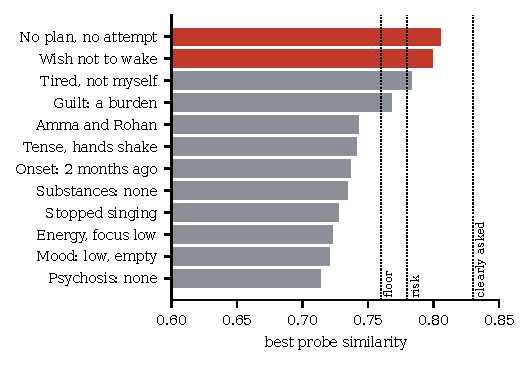
\includegraphics[width=0.85\linewidth]{fig_recall_example.pdf}
\caption{The twelve closest memories for ``Have you ever felt like you'd be better off not being around?'' (depression case). Red: risk memories.
Dotted lines: the cut-offs. The right answer (the death wish) is second, 0.005 behind a related memory.}
\label{fig:example}
\end{figure}

\textbf{Locks after matching, and ``clearly asked''.} Matching does not look at trust; the open/locked split is applied afterwards. A cleverly
reworded question about a locked memory therefore still produces only a discomfort signal, and locked text never enters the prompt. A stricter
level marks what the doctor \emph{clearly} asked about: a keyword hit or a similarity of at least 0.83. Only this level may force the patient to
disclose an unlocked risk memory; an ordinary match never does.

\textbf{Hand-set heads.} For five risk topics (suicidal thoughts, plans, means, harm to others, withdrawal) the first author and an AI assistant wrote 10--17
example questions from standard clinical phrasing (Appendix~\ref{app:heads}). Each topic's weight vector is the normalised mean of their vectors,
\begin{equation}
w_k = \bar{e}_k / \lVert \bar{e}_k \rVert, \qquad \text{match if } w_k^\top e(u) \ge 0.76,
\end{equation}
and a question that passes is ``clearly asked'' for the memories tagged with that topic. There is no training and no model-made label; the
threshold was picked from the dev curve (dev risk recall 96.0\% at 15.9\% false hits).

\subsection{Baselines}
\textbf{BM25} \cite{robertson2009bm25} ($k_1=1.5$, $b=0.75$) indexes every probe as a document with the same stemming, and scores a memory by its best
probe. \textbf{Five small encoders} replace bge-small with all-MiniLM-L6-v2 \cite{wang2020minilm}, e5-small-v2 (with its ``query:'' prefix)
\cite{wang2022e5}, gte-small \cite{li2023gte}, bge-small-en-v1.5 and bge-base-en-v1.5 \cite{xiao2023cpack}, each scoring a memory by its best
probe over the same probes. The \textbf{hybrid's score} for threshold-free metrics is its similarity plus 0.05 per tag point, with any tag hit ranked
above any embedding-only score, which is the order its rules use. Because cut-offs belong to a model, each scored method also gets an
\textbf{operating point}: the lowest cut-off whose dev-half risk false-hit rate is at most the deployed hybrid's (12.7\%), reported on the test
half.

\textbf{Zero-shot language model.} The patient's own model, Gemma 4 E4B (4-bit, llama.cpp, the same laptop), receives the case's memories with
their ids and full text and the doctor's line, and returns the ids of the memories the line asks about (at most three) through a JSON schema;
temperature 0. It yields one operating point and a latency. We timed it with the judge model unloaded, as in a live session.

\textbf{Cascade.} The hybrid screens every question on the processor; only questions whose best risk score reaches a floor go to the language
model, which then decides. The floor is the highest that keeps dev-half risk recall within two points of the model alone.

\textbf{Probe quality filter.} 46\% of the generated probes for risk memories contain no risk word. We drop those, using a fixed word list (death,
dying, kill, harm, hurt, plan, pills, rope, jump, overdose, better off, not be here, wake up, fits, shaking, withdrawal, anger, hit, safe and
related forms; \numFilterDropped{} of \numFilterTotal{} probes), and re-run every probe-based method.

\subsection{Use of language models}
All local models ran through llama.cpp (4-bit Q4\_K\_M) on one laptop between 13 and 19 November 2026. The original benchmark was written by
an AI agent (Claude, Anthropic, through Claude Code) that saw only the memory descriptions. Qwen3.5-9B wrote the generated probes and the
classifier's training lines (temperature 0.95) and labelled the training lines (temperature 0); Qwen3.5-4B and Gemma 4 E2B wrote the two
further test sets (temperature 0.9, fixed seeds); Gemma 4 E4B is the zero-shot classifier (temperature 0, JSON schema). All prompts are in
\texttt{tools/recall\_writer.py}, \texttt{tools/recall\_baselines.py} and \texttt{tools/brain/gen\_lines.py} in the code repository. The AI
assistant (Claude Opus 5.5, Anthropic, through Claude Code, October--November 2026) also drafted the analysis scripts and much of the text of
this manuscript under the authors' direction. The authors reviewed the text, checked every reported number against the saved results, and
take responsibility for the content.

\section{Results}\label{sec:results}

\subsection{The deployed matcher on the test half}
Table~\ref{tab:test} gives the deployed rules. The hybrid doubled risk recall compared with keywords, at about two and a half times the wrong
risk matches; hand-set heads added 5.2 points of recall for 6.0 points of wrong matches. A bootstrap over the 77 risk pairs gives a 95\% interval
of 62.3--81.8\% for the hybrid's risk recall: far from a 95\% target. Every wrong match on a ``none'' line came from a keyword (``tell me'',
``morning'' in ``Good morning''); the sentence model added none. Matching took 2--3\,ms per question on the processor.

\begin{table}[t]
\caption{Deployed rules on the test half (never used for tuning)}
\label{tab:test}
\footnotesize
\begin{tabular*}{\linewidth}{@{\extracolsep{\fill}}lcccc@{}}
\toprule
Method & All & Risk & Risk false hits & ``None'' hit\\
\midrule
Keywords only & 41.3\% & 35.1\% & 6.1\% & 22.7\%\\
Hybrid & 73.3\% & 72.7\% & 15.2\% & 22.7\%\\
Hybrid + hand-set heads & 74.9\% & 77.9\% & 21.2\% & 22.7\%\\
\bottomrule
\end{tabular*}
\end{table}

Recall was lowest for the alcohol case (61.2\%), whose memories are often asked about in slang and euphemism (``How many pegs would you have on a
typical day?''), and for lines the writer marked hard (57.1\% against 92.1\% for easy lines; keywords 19.5\% and 66.7\%). Supplementary Section~S1
gives the breakdown by case, difficulty, kind of memory and risk memory.

\subsection{The encoder is not the bottleneck}
Table~\ref{tab:baselines} and Fig.~\ref{fig:pr} compare the methods. Every encoder ranked risk memories far better than keyword tags (risk AUROC
0.88--0.91 against 0.66), and BM25 over the same probes came close (0.86). Their intervals overlap: bge-base, three times larger than bge-small,
gained 0.007 AUROC. At the matched operating point the encoders found 66--78\% of test-half risk questions, and the method with the highest
recall (bge-base, 77.9\%) also had the most false hits (17.6\%): the dev-set cut-off transferred unevenly. Ranking was already good: the correct
memory had the highest similarity 73.3\% of the time, was in the top three 92.3\% and in the top five 96.4\%. What fails is the decision of how
far down the list to accept. Correct pairs have a median similarity of 0.82, but 11.2\% of non-risk questions score at least 0.78 against some risk
memory, so no single cut-off separates them (Supplementary Section~S2).

\begin{table*}[t]
\caption{Methods on the test half: threshold-free metrics and an operating point matched on the dev half}
\label{tab:baselines}
\scriptsize
\begin{tabular*}{\textwidth}{@{\extracolsep{\fill}}lcccc@{}}
\toprule
Method & \begin{tabular}{@{}c@{}}Risk AUROC\\(95\% CI)\end{tabular} & \begin{tabular}{@{}c@{}}Risk AUPRC\\(95\% CI)\end{tabular} & Recall & False hits\\
\midrule
Keyword tags (v0) & 0.661 (0.61--0.72) & 0.277 (0.20--0.38) & 35.1\% & 5.3\%\\
BM25, probes & 0.863 (0.82--0.90) & 0.518 (0.42--0.63) & 55.8\% & 20.3\%\\
MiniLM-L6 (22M) & 0.888 (0.85--0.93) & 0.604 (0.51--0.70) & 70.1\% & 14.4\%\\
e5-small-v2 (33M) & 0.882 (0.84--0.93) & 0.653 (0.57--0.74) & 71.4\% & 10.7\%\\
gte-small (33M) & 0.906 (0.87--0.94) & 0.612 (0.53--0.70) & 72.7\% & 13.9\%\\
bge-small (33M) & 0.900 (0.87--0.93) & 0.620 (0.54--0.71) & 66.2\% & 13.4\%\\
bge-base (109M) & 0.907 (0.87--0.94) & 0.638 (0.56--0.73) & 77.9\% & 17.6\%\\
Hybrid (deployed) & 0.898 (0.86--0.93) & 0.552 (0.47--0.66) & 67.5\% & 13.9\%\\
\midrule
Gemma 4 E4B, zero-shot & -- & -- & 94.8\% & 4.8\%\\
Cascade (hybrid, Gemma) & -- & -- & 93.5\% & 3.7\%\\
\bottomrule
\end{tabular*}

\par\vspace{1mm}\raggedright\scriptsize AUROC and AUPRC over (question, risk memory) pairs of the question's case (prevalence 0.098); over all
memories, AUROC ranged from 0.69 (tags) and 0.86 (BM25) to 0.91--0.94 (encoders and hybrid). Risk recall and false hits use the cut-off whose dev-half risk false-hit rate is at most the deployed hybrid's (12.7\%); the deployed
rules themselves give 72.7\% and 15.2\% (Table~\ref{tab:test}). The language model gives one operating point, so no curve.
\end{table*}

\begin{figure}[t]
\centering
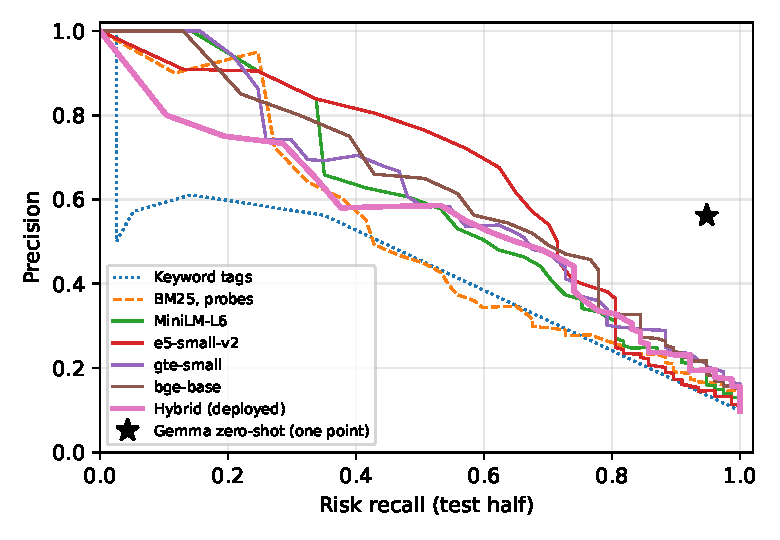
\includegraphics[width=0.85\linewidth]{fig_pr_curves.pdf}
\caption{Precision against risk recall on the test half, over (question, risk memory) pairs. The star is the zero-shot language model.}
\label{fig:pr}
\end{figure}

\subsection{The patient's own model recognises far more}
Used as a zero-shot classifier, Gemma found \numLLMrisk{} of test-half risk questions and wrongly matched \numLLMfalse{} of non-risk ones, better on
both counts than every method above. It needs one model call per question: a median of \numLLMmsMed\,ms (90th percentile \numLLMmsNinety\,ms) on
the laptop's graphics processor, which the patient's own reply also needs, against 2--3\,ms on the processor for the hybrid. Table~\ref{tab:cascade}
shows the cascade: with the floor set on the dev half, it kept \numCasRisk{} recall at \numCasFalse{} false hits while sending \numCasShare{} of
test questions to the model. Raising the floor saves calls quickly but loses recall just as quickly, because many reworded risk questions score
low on every encoder.

\begin{table}[t]
\caption{Cascade on the test half: the hybrid screens, the language model decides (bold: the floor chosen on the dev half)}
\label{tab:cascade}
\footnotesize
\begin{tabularx}{\linewidth}{@{}Yccc@{}}
\toprule
Screen floor & Risk recall & Risk false hits & Lines sent to the LLM\\
\midrule
0.50 & 94.8\% & 4.8\% & 100\%\\
0.55 & 94.8\% & 4.8\% & 99\%\\
0.60 & 94.8\% & 4.8\% & 96\%\\
0.65 & 94.8\% & 4.3\% & 86\%\\
\textbf{0.70} & \textbf{93.5\%} & \textbf{3.7\%} & \textbf{63\%}\\
0.75 & 83.1\% & 2.7\% & 41\%\\
0.80 & 63.6\% & 2.1\% & 26\%\\
0.85 & 48.1\% & 1.6\% & 19\%\\
0.90 & 42.9\% & 1.6\% & 17\%\\
\bottomrule
\end{tabularx}

\end{table}

\subsection{Filtering the generated probes}
Table~\ref{tab:filter} re-runs the probe-based methods without the generated risk probes that contain no risk word. Some of the dropped probes
were plainly off-topic (``Before we continue, could you tell me a bit about how you have been sleeping lately?'' was listed as a probe for the death
wish), which explains why sleep questions had matched suicide memories. The filter barely moved the threshold-free metrics; with the deployed rules
it cut risk false hits on both halves but also cost recall, because some dropped probes were fair indirect questions (``Have you felt that life has
lost its meaning?'').

\begin{table*}[t]
\caption{Effect of the probe quality filter (test half unless stated)}
\label{tab:filter}
\scriptsize
\begin{tabularx}{\textwidth}{@{}Ycccccc@{}}
\toprule
Method & \multicolumn{2}{c}{Risk AUROC} & \multicolumn{2}{c}{Risk recall} & \multicolumn{2}{c}{Risk false hits}\\ & all & filtered & all & filtered & all & filtered\\
\midrule
BM25, probes & 0.863 & 0.864 & 55.8\% & 58.4\% & 20.3\% & 20.3\%\\
MiniLM-L6 (22M) & 0.888 & 0.888 & 70.1\% & 71.4\% & 14.4\% & 18.7\%\\
e5-small-v2 (33M) & 0.882 & 0.868 & 71.4\% & 71.4\% & 10.7\% & 13.9\%\\
gte-small (33M) & 0.906 & 0.903 & 72.7\% & 72.7\% & 13.9\% & 14.4\%\\
bge-small (33M) & 0.900 & 0.898 & 66.2\% & 67.5\% & 13.4\% & 12.3\%\\
bge-base (109M) & 0.907 & 0.906 & 77.9\% & 72.7\% & 17.6\% & 15.0\%\\
Hybrid (deployed) & 0.898 & 0.896 & 67.5\% & 71.4\% & 13.9\% & 14.4\%\\
\midrule
Deployed match rules (dev half) & -- & -- & 90.7\% & 86.7\% & 12.7\% & 7.6\%\\
Deployed match rules (test half) & -- & -- & 72.7\% & 68.8\% & 15.2\% & 12.1\%\\
\bottomrule
\end{tabularx}

\end{table*}

\subsection{A new writer, and code-mixed questions}
Table~\ref{tab:writers} repeats the comparison on the two further test sets. The gap between the deployed rules and the zero-shot model held, and
widened: on the sets written by Qwen3.5-4B and Gemma 4 E2B the zero-shot model found \numWQwenLLM{} and \numWGemmaLLM{} of risk questions with
7.9\% and 6.8\% false hits, while the deployed rules found \numWQwenDep{} and \numWGemmaDep, well below their 72.7\% on the original test
half. The original benchmark therefore flattered the matcher, whose probes and cut-offs were shaped on the first writer's dev half. The
Gemma-written set may favour the Gemma classifier, but the Qwen-written set, which shares a family with the generated probes and so should
favour the matcher, shows the same gap. Among the encoders, gte-small and bge-base ranked best on both sets (risk AUROC 0.81--0.85), and BM25's
dev-matched cut-off transferred badly (55.6\% and 71.4\% false hits). Table~\ref{tab:hinglish} gives risk
recall on the code-mixed lines alone: 16 risk pairs per writer, so the numbers are rough, but the deployed rules found 31.2\% and 43.8\% and
the zero-shot model 87.5\% on both. Every encoder here was trained mainly on English, so these lines test a case the deployed matcher was never
designed for, and one that Indian students will produce.

\begin{table*}[t]
\caption{The methods on two further test sets written by other local models (cut-offs from the original dev half)}
\label{tab:writers}
\scriptsize\setlength{\tabcolsep}{3pt}
\begin{tabular*}{\textwidth}{@{\extracolsep{\fill}}lcccccc@{}}
\toprule
& \multicolumn{3}{c}{Written by Qwen3.5-4B} & \multicolumn{3}{c}{Written by Gemma 4 E2B}\\ Method & AUROC & Recall & FH & AUROC & Recall & FH\\
\midrule
Keyword tags (v0) & 0.693 & 44.5\% & 6.0\% & 0.566 & 18.4\% & 12.3\%\\
BM25, probes & 0.780 & 87.0\% & 55.6\% & 0.731 & 78.7\% & 71.4\%\\
bge-small (33M) & 0.789 & 33.6\% & 6.9\% & 0.785 & 37.6\% & 22.7\%\\
bge-base (109M) & 0.808 & 45.9\% & 11.6\% & 0.824 & 62.4\% & 25.0\%\\
gte-small (33M) & 0.826 & 50.0\% & 7.4\% & 0.846 & 48.9\% & 17.3\%\\
Hybrid (deployed) & 0.834 & 54.8\% & 11.1\% & 0.782 & 41.1\% & 29.1\%\\
\midrule
Deployed match rules & -- & 58.9\% & 9.9\% & -- & 47.5\% & 25.5\%\\
Gemma 4 E4B, zero-shot & -- & 87.7\% & 7.9\% & -- & 91.5\% & 6.8\%\\
\bottomrule
\end{tabular*}

\par\vspace{1mm}\raggedright\scriptsize AUROC over (question, risk memory) pairs; Recall and FH (risk false hits) at the cut-off matched on the
original dev half, as in Table~\ref{tab:baselines}.
\end{table*}

\begin{table}[t]
\caption{Risk recall on the code-mixed Hindi--English lines of the two further sets}
\label{tab:hinglish}
\scriptsize
\begin{tabularx}{\linewidth}{@{}Ycccc@{}}
\toprule
Writer & Hinglish lines & Risk pairs & Deployed rules & Gemma zero-shot\\
\midrule
Qwen3.5-4B & 70 & 16 & 31.2\% & 87.5\%\\
Gemma 4 E2B & 49 & 16 & 43.8\% & 87.5\%\\
\bottomrule
\end{tabularx}

\end{table}

\subsection{Why questions were missed}
Of the 21 risk pairs the deployed hybrid missed on the test half, 8 matched nothing, 8 matched only a non-risk memory, and 5 matched a different
risk memory (which does little harm: a locked risk match still makes the patient evasive). Table~\ref{tab:misses} groups them by type. A real
clinician would recognise all of them as risk questions.

\begin{table}[t]
\caption{Missed risk questions on the test half, by type}
\label{tab:misses}
\scriptsize
\begin{tabularx}{\linewidth}{@{}lY@{}}
\toprule
Type & Real example (expected memory)\\
\midrule
Euphemism & ``Do you ever feel like you just want it all to stop?'' (death wish)\\
Situation, not thought & ``If these feelings got worse tonight, do you think you would do anything about them?'' (no plan)\\
Open question & ``In your lowest moment recently, what was going through your mind?'' (passive death thought)\\
Other people's angle & ``Have you ever thought your family would manage better if you weren't there?'' (passive death thought)\\
Matched a nearby topic & ``Have you googled anything about overdoses?'' $\to$ substance use (no means)\\
Indirect action & ``Have you ever swallowed something or cut yourself in a bad moment?'' (no plan or means)\\
Physical wording & ``Do things ever get physical at home?'' $\to$ consequences (anger at home)\\
\bottomrule
\end{tabularx}
\end{table}

\subsection{Two negative results}
\textbf{Tuning for recall alone is unsafe.} The chosen setting scored 90.7\% risk recall on the dev half and 72.7\% on the test half. An earlier
setting, tuned after probes inspired by dev-half misses had been added, scored 98.7\% on dev and the same 72.7\% on test: about 75 risk pairs,
used twice, are enough to fit the dev half without improving on new questions. An automatic re-tune that maximised dev risk recall reached 100\%
but matched 36.9\% of non-risk dev questions to a risk memory (37.6\% on test; Table~\ref{tab:sweep}). In held-out conversations the patient then
treated ``How have you been sleeping, and how is your appetite?'' as a suicide question, and mentioned the death wish unasked in 3 of 98 turns.
Separating ``matched'' from ``clearly asked'' and capping wrong risk matches fixed it. Every step down in the risk cut-off buys a few points of
recall for several points of wrong matches; reaching 95\% on new questions would need a cut-off below 0.72, where a third of ordinary questions
already look like risk questions.

\begin{table}[t]
\caption{Moving the risk cut-off (other settings as shipped)}
\label{tab:sweep}
\footnotesize
\begin{tabular*}{\linewidth}{@{\extracolsep{\fill}}lcccc@{}}
\toprule
& \multicolumn{2}{c}{Dev half} & \multicolumn{2}{c}{Test half}\\
Risk cut-off & Recall & False hits & Recall & False hits\\
\midrule
0.72 & 100\% & 34.4\% & 89.6\% & 34.5\%\\
0.74 & 98.7\% & 23.6\% & 83.1\% & 25.5\%\\
0.76 & 93.3\% & 17.8\% & 76.6\% & 19.4\%\\
\textbf{0.78 (shipped)} & \textbf{90.7\%} & \textbf{12.7\%} & \textbf{72.7\%} & \textbf{15.2\%}\\
0.80 & 81.3\% & 8.9\% & 70.1\% & 12.7\%\\
0.82 & 81.3\% & 5.1\% & 66.2\% & 9.7\%\\
\midrule
Recall-only tune & 100\% & 36.9\% & 84.4\% & 37.6\%\\
\bottomrule
\end{tabular*}
\end{table}

\textbf{A classifier trained on generated labels lost.} A language model wrote 3,301 doctor lines in the voices of an experienced psychiatrist, a
nervous student and a tester trying to break the simulator, plus 369 lines from the developer's own sessions; a judge from another model family
(Qwen3.5-9B) labelled each with its topics and moves. The judge agreed with the topic each generated line was written for only 50.1\% of the time
(38.8\% for the tester's lines). Logistic-regression heads on the frozen sentence vector read the \emph{manner} of a line better than word
patterns overall (micro-F1 0.32 against 0.20) but read its \emph{topic} worse than the live language-model tagger (0.66 against 0.69). A patient
version using them scored lower in held-out conversations and was not shipped. With labels this noisy, a learned model cannot beat simple rules,
and a few hundred hand-checked labels are worth more than thousands of generated ones (Supplementary Section~S3).

\subsection{What a missed match costs in conversation}
Our companion manuscript asked every test-half risk question as the second turn of a short conversation that starts with enough
trust for the memory to be open. The patient failed to disclose in \numRPmissVtwo{} of cases; \numRPmissNoRecVtwo{} of questions the hybrid did not
match went undisclosed, against \numRPmissRecVtwo{} of those it did. A missed match is therefore not only a benchmark error: it is a risk question
the patient may answer as if it were small talk.

\section{Discussion}\label{sec:disc}
\textbf{What we learned.} Comparing questions with example questions, not with the memory's statement, is the step that matters most for small
encoders; after that, the choice among five small encoders, or BM25 over the same probes, changes little. Ranking is good; deciding where to cut is
hard, and cut-offs tuned on a reused dev half do not transfer. A 4-billion-parameter language model, asked directly, recognises reworded risk
questions far better than any cut-off on an encoder, at the cost of hundreds of milliseconds and a share of the graphics processor on every
screened turn. For a spoken patient that has to start talking within about two seconds, a cascade is the practical compromise, and the
\numCasShare{} of questions it sends to the model is the cost of near-model recall.

\textbf{Why not just ask the language model?} Because the call is not free: in the deployed patient it would add to every turn whose question
looks like risk, compete with the patient's own reply for the graphics processor, and still need the trust locks and the ``clearly asked''
distinction applied in code afterwards. The model also sees every memory's text in this design, including locked ones; since only ids come back
and the call is separate from the reply, nothing locked reaches the patient's prompt, but the separation has to be kept by code. Our results argue
that it is worth that cost on risk questions.

\textbf{Limitations.} All test questions were written by language models, never by students or clinicians, so their phrasing may be more
regular than a nervous student's. Labels came from the writers alone and were not checked by a person. About 75
risk pairs per half make each recall figure uncertain by several points. The zero-shot prompt was written once and not tuned; a tuned prompt might
do better, and a different model might do worse. Latency was measured on one high-end laptop. The cases are drafts that a psychiatrist must
still review. Only one variety of English was tested.

\section{Conclusion}
Matching a reworded risk question to a patient's memory is easy to rank and hard to decide. On a blind benchmark, small encoders and BM25 over
example questions ranked well but, with cut-offs from a tuning half, found about three in four risk questions on that writer's test half and
only about half on questions from two new writers; the patient's own language model, asked directly, found \numLLMrisk{}, and close to nine in
ten on the new writers' questions. A cascade gets most of that recall while calling the model on fewer turns. The benchmark, its split and the two further
sets are public with the code.

\begin{appendices}
\section{Instructions given to the benchmark writer}\label{app:writer}
The writer received, for each case: the patient's name, age and situation; for each memory its id, its kind (complaint, symptom, history, risk,
social, belief) and a one-line description of what the patient knows; and these rules: write lines a real doctor might say to this patient; at least
4 per memory and 12 per risk memory; mix textbook, gentle and indirect, clumsy and leading, colloquial Indian English, and euphemistic phrasings;
most lines should avoid the memory's obvious key words; each line must make sense on its own; label each line with every memory it asks about, and
nothing more; include greetings, small talk and empathy-only lines that ask about nothing; mark hard lines. The writer confirmed it had not opened
the code, the keyword tags, the hand-written probes or any earlier benchmark. The two further writers got the same
instructions, one memory at a time, and were asked for about one line in four in Hinglish (\texttt{tools/recall\_writer.py}).

\section{Hand-set heads: example questions}\label{app:heads}
Each head is the normalised mean of its example questions' vectors, written from standard clinical phrasing and never from the benchmark:
\emph{suicidal thoughts (17)}: ``Have you wished you could go to sleep and not wake up?'', ``Do you sometimes feel everyone would be better off
without you?''; \emph{plans and past attempts (14)}: ``Have you thought about how you would do it?'', ``Can you keep yourself safe if you go home
today?''; \emph{means (12)}: ``Have you been saving up medicines?'', ``Is your home safe for you right now?''; \emph{harm to others}: ``Has anyone at
home been afraid of you?'', ``Have arguments ever got physical?''.
\end{appendices}

\backmatter

\bmhead{Supplementary information}
Supplementary material (\texttt{supplementB.pdf}) gives recall by case, difficulty, kind of memory and risk memory (S1), rank and probe ablations,
similarity distributions and the cut-offs (S2), and the classifier's data and results (S3).

\section*{Statements and Declarations}
\begin{itemize}
\item \textbf{Funding:} The authors did not receive support from any organization for the submitted work.
\item \textbf{Competing interests:} F.K.M.\ develops Rapport, which is open source. S.S.\ has no competing interests to declare.
\item \textbf{Ethics approval:} Not applicable. The study involved no human participants and no patient data.
\item \textbf{Consent to participate and to publish:} Not applicable.
\item \textbf{Data availability:} The benchmark, its split, the two further test sets, the probes and every method's per-question output are
archived on Zenodo (version 0.3.0, \url{https://doi.org/10.5281/zenodo.24367081}) and available from the authors on request.
\item \textbf{Code availability:} The code, including \texttt{tools/recall\_bench.py}, \texttt{tools/recall\_baselines.py} and
\texttt{tools/recall\_writer.py}, is archived in the same Zenodo record (\url{https://doi.org/10.5281/zenodo.24367081}) under the Apache License 2.0 and is available on request.
\item \textbf{Author contributions:} Both authors contributed to the study conception and design, the analysis and the manuscript, and
read and approved the final manuscript.
\item \textbf{Use of AI tools:} Described under ``Use of language models'' in the Methods.
\end{itemize}

\bibliography{../shared/refs}

\end{document}
